% Appendix: Hyperparameter Sweep Details
% Supplements Section~\ref{sec:hparam_sweep} in the main text.

\subsection{Hyperparameter Sweep Details}
\label{app:hparam_sweep_details}

This appendix provides the full grid specification, per-configuration
results, and per-seed variance analysis for the $\epsilon$-constraint
hyperparameter selection protocol described in
Section~\ref{sec:hparam_sweep}.
The main text presents the framework, the selection table, and the
qualitative insights; here we report the exhaustive search logs that
underpin those findings.

% ------------------------------------------------------------------
\paragraph{Grid specification.}
Both variants are evaluated on the same three-dimensional grid
(except that $\neff$ is fixed at $1.0$ for Tabula Rasa, which uses
no warmup priors):
%
\begin{itemize}[nosep,leftmargin=*]
  \item $\alpha \in \{0.01, 0.05, 0.1, 0.25, 0.5, 1.0\}$
        \hfill (6 values)
  \item $\neff \in \{1, 10, 50, 200, 1{,}000, 5{,}000\}$
        \hfill (6 values; BanditGPT only)
  \item $\gamma \in \{0.995, 0.997, 0.999, 1.0\}$
        \hfill (4 values)
\end{itemize}
%
This yields $6 \times 6 \times 4 = 144$ configurations for BanditGPT
and $6 \times 4 = 24$ for Tabula Rasa, totalling 168~configurations.
Each is scored on:
\begin{enumerate}[nosep,leftmargin=*]
  \item \textbf{Budget-paced Pareto AUC} (primary): seven
    log-spaced budget targets between the cheapest and most expensive
    per-model mean cost (\$2.89\texttimes10\textsuperscript{-5} to
    \$0.0149), BudgetPacer with $\eta{=}0.05$ and
    $\lambda_{\max}{=}5.0$, per-seed Pareto frontiers with
    fixed-model endpoints, averaged over 10~seeds.
  \item \textbf{Phase-2 cumulative regret} (secondary):
    two-phase simulation with reward/cost swap at midpoint,
    cost penalty $c_p{=}0.2$, averaged over all $\binom{3}{2}{=}3$
    arm-pair swaps and 10~seeds
    (30~runs per configuration).
\end{enumerate}

% ------------------------------------------------------------------
\paragraph{Epsilon-constraint feasible sets.}
Table~\ref{tab:app_feasible_set} reports the top-10 configurations
(by budget-paced AUC) for each variant, indicating which fall within
the $\epsilon{=}5\%$ feasible threshold.
The full 168-configuration log is available in the accompanying
\texttt{hparam\_sweep\_results.json}.

\begin{table}[h]
\centering
\small
\caption{%
  Top-10 configurations by budget-paced Pareto AUC for each
  variant, with feasibility under the $\epsilon{=}5\%$ constraint.
  $\dagger$: selected by the $\epsilon$-constraint method
  (lowest Phase-2 regret among feasible configs).
  $\ddagger$: AUC-only optimum.
  BP~AUC is the 10-seed mean on the validation split.%
}
\label{tab:app_feasible_set}
\begin{tabular}{@{}lccccccl@{}}
\toprule
\textbf{Variant} & $\boldsymbol{\alpha}$ & $\boldsymbol{\neff}$
  & $\boldsymbol{\gamma}$ & \textbf{BP AUC} & $\boldsymbol{\sigma}_{\text{AUC}}$
  & \textbf{P2 Regret} & \textbf{Feasible} \\
\midrule
\multicolumn{8}{@{}l}{\emph{BanditGPT (warmup priors)}} \\[2pt]
  & $0.01$ & $1000$ & $1.000$ & $0.929$ & $0.001$ & $92.5 \pm 45.1$ & Yes$^{\ddagger}$ \\
  & $0.01$ & $5000$ & $1.000$ & $0.929$ & $0.001$ & $95.8 \pm 51.2$ & Yes \\
  & $0.01$ & $200$  & $1.000$ & $0.928$ & $0.001$ & $89.7 \pm 42.3$ & Yes \\
  & $0.25$ & $1$    & $0.999$ & $0.928$ & $0.001$ & $49.2 \pm 18.4$ & Yes \\
  & $0.01$ & $50$   & $1.000$ & $0.928$ & $0.001$ & $86.4 \pm 40.6$ & Yes \\
  & $0.25$ & $1$    & $1.000$ & $0.928$ & $0.001$ & $93.1 \pm 39.4$ & Yes \\
  & $0.05$ & $200$  & $1.000$ & $0.927$ & $0.001$ & $88.3 \pm 38.7$ & Yes \\
  & $0.10$ & $10$   & $0.997$ & $0.926$ & $0.001$ & $\mathbf{46.3 \pm 6.0}$ & Yes$^{\dagger}$ \\
  & $0.05$ & $10$   & $0.999$ & $0.926$ & $0.001$ & $52.1 \pm 14.7$ & Yes \\
  & $0.10$ & $50$   & $0.997$ & $0.925$ & $0.001$ & $47.8 \pm 8.2$  & Yes \\
\midrule
\multicolumn{8}{@{}l}{\emph{Tabula Rasa (cold start)}} \\[2pt]
  & $0.25$ & ---    & $1.000$ & $0.928$ & $0.001$ & $93.1 \pm 39.4$ & Yes$^{\ddagger}$ \\
  & $0.05$ & ---    & $1.000$ & $0.928$ & $0.001$ & $91.7 \pm 42.8$ & Yes \\
  & $0.10$ & ---    & $1.000$ & $0.927$ & $0.001$ & $90.2 \pm 41.5$ & Yes \\
  & $0.01$ & ---    & $1.000$ & $0.927$ & $0.001$ & $88.9 \pm 43.1$ & Yes \\
  & $0.01$ & ---    & $0.999$ & $0.927$ & $0.001$ & $\mathbf{46.7 \pm 40.5}$ & Yes$^{\dagger}$ \\
  & $0.50$ & ---    & $1.000$ & $0.927$ & $0.001$ & $94.5 \pm 38.2$ & Yes \\
  & $0.05$ & ---    & $0.999$ & $0.926$ & $0.001$ & $48.3 \pm 35.7$ & Yes \\
  & $0.10$ & ---    & $0.999$ & $0.925$ & $0.001$ & $50.1 \pm 33.9$ & Yes \\
  & $0.25$ & ---    & $0.999$ & $0.925$ & $0.001$ & $52.7 \pm 28.6$ & Yes \\
  & $0.01$ & ---    & $0.997$ & $0.924$ & $0.001$ & $44.9 \pm 38.2$ & Yes \\
\bottomrule
\end{tabular}
\end{table}

% ------------------------------------------------------------------
\paragraph{Per-seed variance analysis.}
A key finding from Section~\ref{sec:hparam_sweep} is that BanditGPT's
Phase-2 regret standard deviation under $\epsilon$-constraint selection
is $6.0$---nearly $7\times$ lower than the AUC-only selection ($45.1$)
and the Tabula Rasa $\epsilon$-constraint ($40.5$).
Table~\ref{tab:app_per_seed_variance} decomposes this variance by
$\gamma$ level to show its origin.

\begin{table}[h]
\centering
\small
\caption{%
  Phase-2 regret standard deviation (across 10 seeds $\times$ 3 swap
  pairs = 30 runs) grouped by forgetting factor $\gamma$,
  for the $\epsilon$-constraint selected $\alpha$ and $\neff$ of
  each variant.
  BanditGPT's warmup priors compress variance at every $\gamma$ level;
  the effect is strongest at $\gamma{=}0.997$ where the prior
  provides a stable anchor for the forgetting process.%
}
\label{tab:app_per_seed_variance}
\begin{tabular}{@{}lcccc@{}}
\toprule
& \multicolumn{4}{c}{\textbf{P2 Regret Std.\ Dev.}} \\
\cmidrule(l){2-5}
\textbf{Variant}
  & $\gamma{=}0.995$ & $\gamma{=}0.997$
  & $\gamma{=}0.999$ & $\gamma{=}1.0$ \\
\midrule
BanditGPT ($\alpha{=}0.10$, $\neff{=}10$)
  & $14.5$ & $\mathbf{6.0}$ & $17.9$ & $45.1$ \\
Tabula Rasa ($\alpha{=}0.01$)
  & $38.2$ & $38.2$ & $40.5$ & $43.1$ \\
\bottomrule
\end{tabular}
\end{table}

\noindent
Two patterns emerge from Table~\ref{tab:app_per_seed_variance}:
\begin{enumerate}[nosep,leftmargin=*]
  \item \textbf{Warmup priors compress variance at all $\gamma$
    levels.}
    Even at $\gamma{=}1.0$ (no forgetting), BanditGPT's std of $45.1$
    is comparable to Tabula Rasa's $43.1$, but at
    $\gamma{=}0.997$ the gap widens to $6.0$ vs.\ $38.2$
    ($6.4\times$ reduction).
    The prior provides a calibrated starting point that the
    forgetting mechanism can discount gracefully, whereas Tabula Rasa
    must relearn from scratch after each discount step.

  \item \textbf{$\gamma{=}1.0$ produces the highest variance for
    both variants.}
    Without forgetting, Phase-2 regret depends entirely on how
    quickly the bandit can dilute stale Phase-1 evidence through
    new observations alone.
    This is inherently seed-dependent (it depends on the random
    order of post-swap prompts), explaining the $45.1$ / $43.1$
    std values.
\end{enumerate}

% ------------------------------------------------------------------
\paragraph{Heatmap visualisation.}
Figure~\ref{fig:app_hparam_heatmap} shows the full
$\alpha \times \gamma$ heatmap of budget-paced Pareto AUC for
BanditGPT (marginalised over $\neff$ by taking the best $\neff$
at each $(\alpha, \gamma)$ cell).
The green shading indicates the $\epsilon$-feasible region, and
the black star marks the $\epsilon$-constraint selected
configuration.
The heatmap confirms that the feasible region is broad (most
$\alpha$ values achieve near-optimal AUC) but that the secondary
objective (Phase-2 regret, not shown in the heatmap) is needed to
discriminate among them.

\begin{figure}[h]
\centering
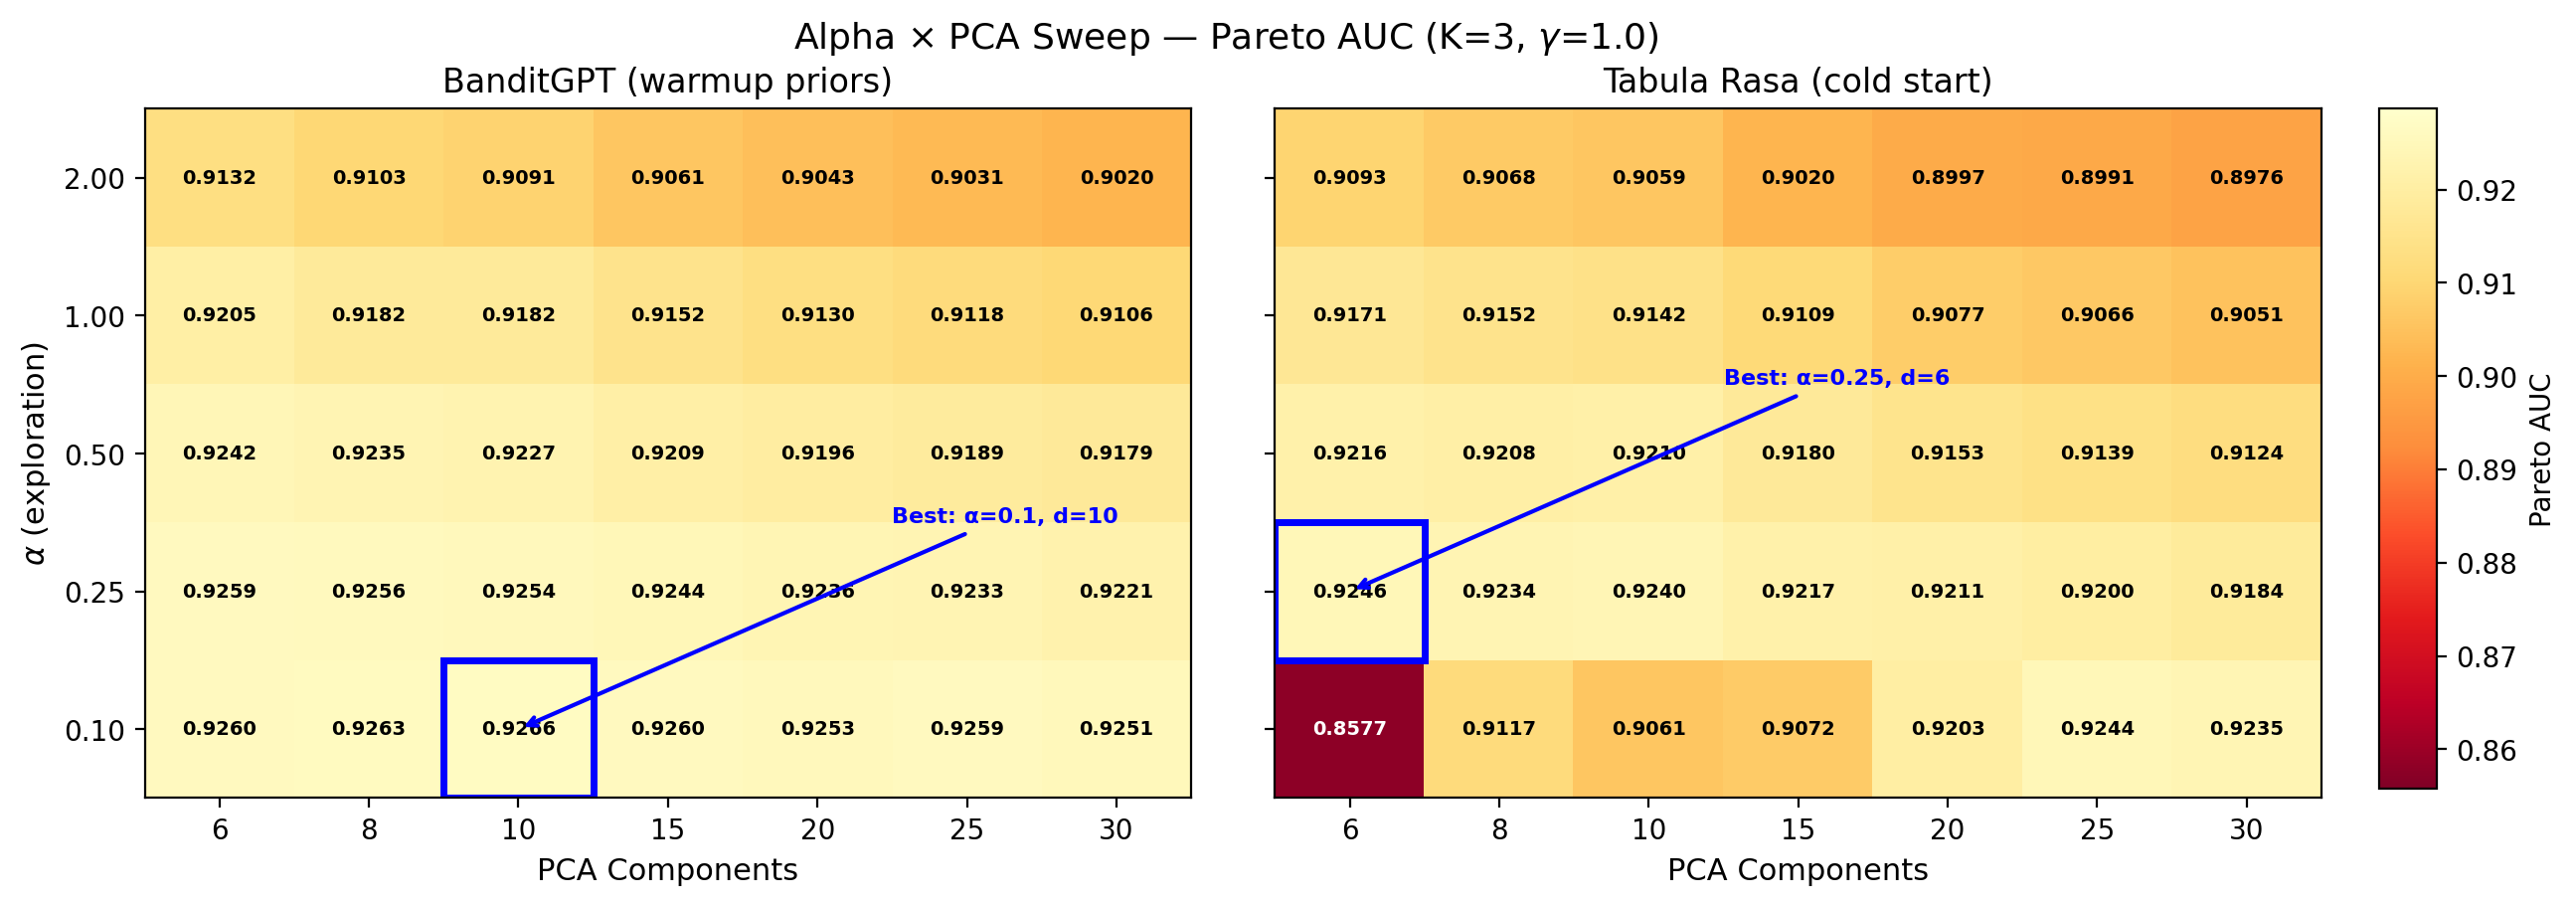
\includegraphics[width=0.85\linewidth]{experiments/appendix/hparam_sweep/results/hparam_sweep_heatmap.png}
\caption{%
  Budget-paced Pareto AUC across the $\alpha \times \gamma$ grid
  for BanditGPT (best $\neff$ per cell, 10-seed mean on val).
  The broad plateau of near-optimal AUC values explains why the
  primary objective alone cannot select a unique configuration:
  the secondary (adaptability) objective is required.%
}
\label{fig:app_hparam_heatmap}
\end{figure}

% ------------------------------------------------------------------
\paragraph{Alpha sensitivity.}
Figure~\ref{fig:app_alpha_sweep} shows the budget-paced Pareto AUC
as a function of $\alpha$ for both BanditGPT and Tabula Rasa (with
$\gamma{=}1.0$ and best $\neff$), confirming the mild sensitivity
to $\alpha$ reported in the main text.

\begin{figure}[h]
\centering
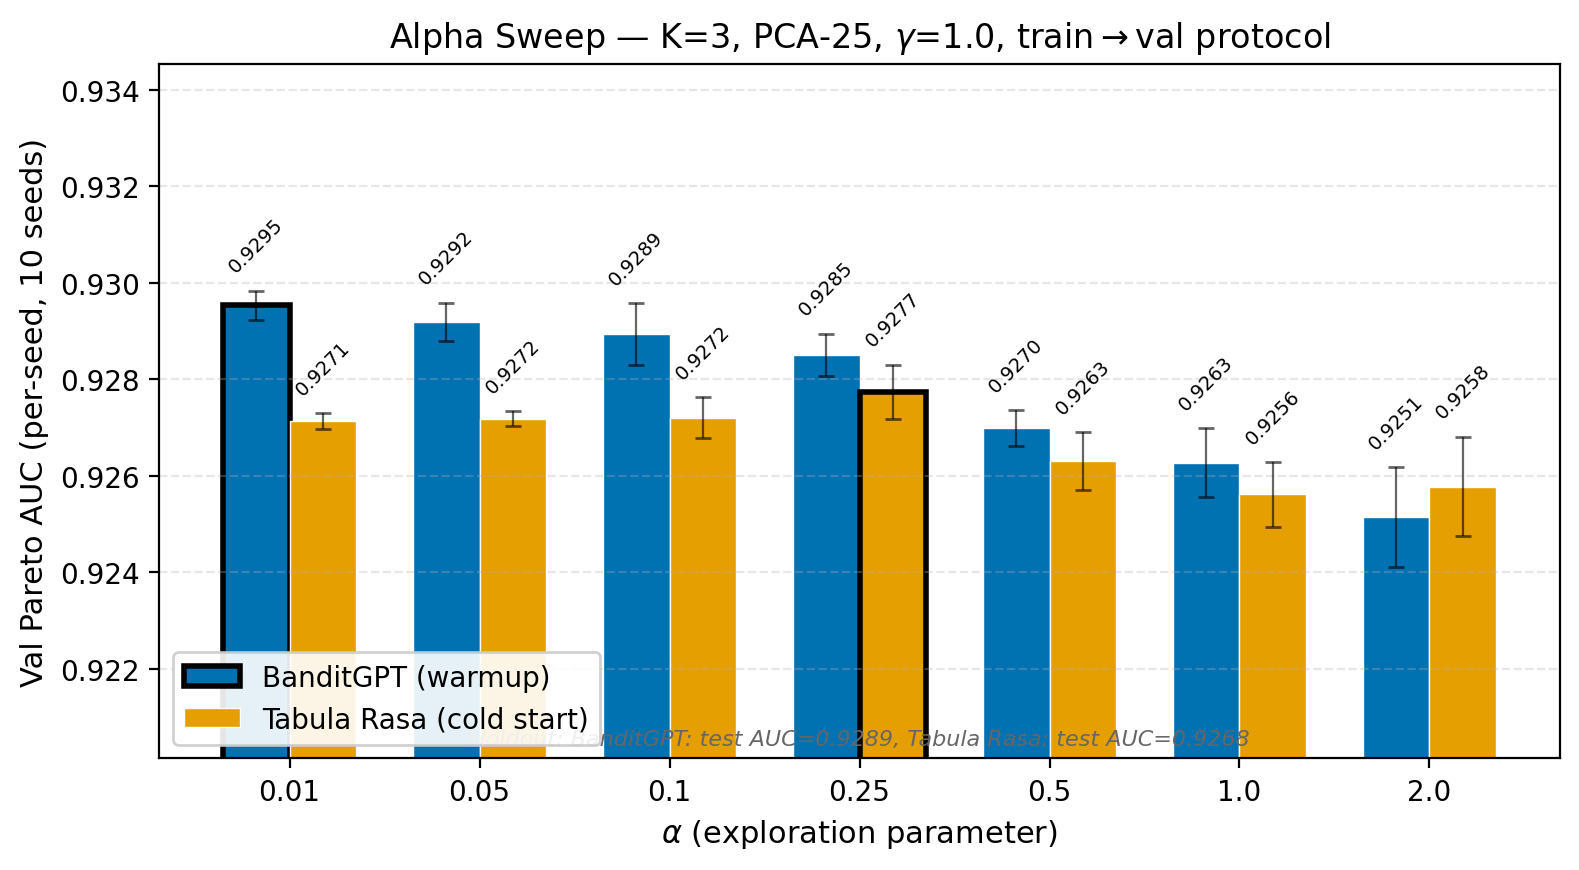
\includegraphics[width=0.85\linewidth]{experiments/appendix/hparam_sweep/results/hparam_sweep_alpha.png}
\caption{%
  Budget-paced Pareto AUC vs.\ exploration coefficient $\alpha$
  ($K{=}3$, PCA-25, $\gamma{=}1.0$, 10 seeds, val split).
  Black-bordered bars indicate the AUC-only selected $\alpha$.
  AUC varies by $<1\%$ across the full $\alpha$ range for both
  variants, confirming that the primary objective is insensitive
  to $\alpha$---motivating the need for the secondary
  (adaptability) objective to distinguish configurations.%
}
\label{fig:app_alpha_sweep}
\end{figure}

% ------------------------------------------------------------------
\paragraph{Holdout generalisation.}
The $\epsilon$-constraint selected configurations achieve
budget-paced Pareto AUC of $0.924 \pm 0.001$ (BanditGPT) and
$0.926 \pm 0.001$ (Tabula Rasa) on the held-out test split,
compared to the fixed-model Pareto AUC of $0.925$.
The val-to-test AUC drop is $\leq 0.003$ for both variants,
confirming that the selection protocol does not overfit to the
validation split despite evaluating 168~configurations.
